\selectlanguage{english}
\def\<#1>{\textit{#1}}


\chapter{Introduction}
\subsection{Overview}

In 1965, Moore predicted, based on observations, that the number of transistors on integrated circuits will double approximately every two years. This was the case for many years after that, with the industry pushing hardware performance forward to meet that goal. Advancements in transistor technology made it possible to integrate more of them in the same silicon chip. Their frequency also increased, presumably doubled every 18 months. At the same time, emerging architecture techniques made it possible to further exploit the continuously increasing cpu power. The use of deeper pipelines superscalar architectures made it possible to increase the operation throughput. Out of order execution and branch predictors helped to make sure that most of the available transistors are utilized, at any given point of the execution. Moreover, hardware manufacturers were able to keep pushing for better performance, without worrying about memory consumption. They were able to achieve higher frequencies fore more transistors, by reducing the voltage supply needed, thus keeping power consumption at controlled levels. In the meantime, cache hierarchies  grew bigger and faster to meet the demands of CPU All those factors made it possible to keep a steady rate of increase in computing power, without any demand for new programming models.

That staggering rate of advancement reached a peak around 2004. At that point, manufacturers were not able to keep making transistors smaller and faster, without sacrificing power consumption. At the same time, memory performance was now too small compared to CPU frequencies, creating and unbridgeable CPU -  memory gap. In order to meet the increasing demands for computer power, computer science shifted towards multicore CPUs. After that point, improvements in performance were no longer achieved exclusively by advancements in architecture, but required fundamental software support. The excess of cores and transistors would mean nothing, if the overlaying software was not able to effectively break execution path down to independent path that could be run in parallel. From user applications, to compilers and operating systems, software needed to be redesigned in way that could exploit the extra cores and the available architecture. Nowadays, the demand for multicore CPUs is no longer an exclusive characteristic of super computers and data centers, but has become rather mainstream, entering the field of desktop computers and embedded systems. Over that time, parallel software techniques have made great steps of progress towards a more efficient utilization of every aspect of modern computer architectures. Despite that progress, parallel programming continues to be a challenging task, and a field of ongoing research.

\section{Flynn's taxonomy}
According to Michael J. Flynn, computer architectures are classified in 4 different categories, according to their instruction and data stream. 

%bulets here

Single Instruction Single Data stream (SISD). 
	A sequential architecture that employs a single processing unit, executing over a single data stream, one operation at a time. 

Single Instruction Multiple Data streams (SIMD).
	An computer  that executes the same command over multiple data streams. An example of such an architecture are Graphic Processor Units (GPS).

Multiple Instruction Single Data streams(MISD).
	A computer where different instructions are executed on the same data stream. This architecture is quite uncommon, and in most cases it is user for false tolerance. An example is an airplane guiding system, where several routines are used and must reach a consensus.

Multiple Instruction Multiple Data streams(MIMD).
	Multiple autonomous processors execute different instructions on different data. Multicore and Distributed Systems are MIMD machines.

%eikona apo wiki http://en.wikipedia.org/wiki/Flynn%27s_taxonomy

\begin{figure}
 \centering
  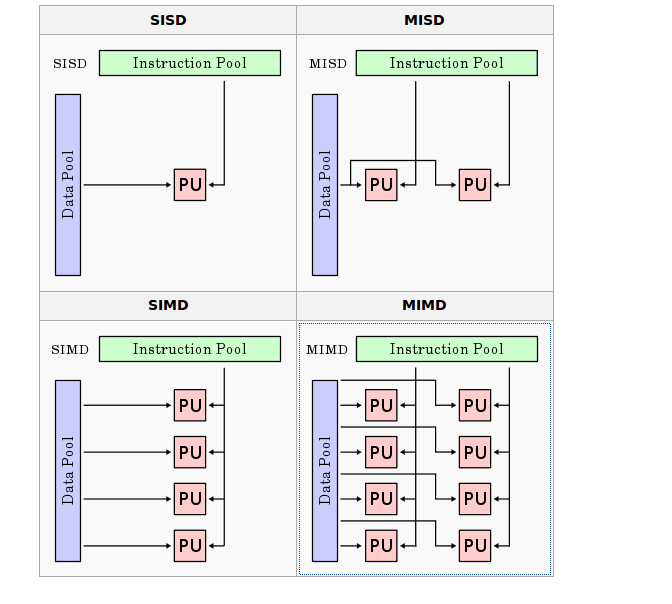
\includegraphics[scale=0.4]{flynsTaxonomy.png}
\caption{Flynn's taxonomy}
\label{Flynn's taxonomy}
\end{figure}

MIMD machines are further classified into 3 categories, according to their address space:

\subsection{shared memory}

In shared memory architectures, every processor has its own hierarchy of cache memory and all processors share the same main memory. Interconnection between processors and memory is typically done through a memory bus, but more sophisticated interconnection networks can be used. Access to memory can take the same amount of time for all processors( Uniform Memory Access -UMA ) or can vary depending on the processor and the memory location( Non Uniform Memory Access) . Non Uniform Memory Access will make memory sharing between adjacent processors fast and reduce bus congestion, but varying access time may make analysis difficult. 

%eikona gia shared memory apo diafanies https://dl-web.dropbox.com/get/SharewithCostas/Lectures/pps-parallel-programming-lec1-Fall2013.pdf?_subject_uid=122896110&w=AAB_Fj7mtgIBvGR3UK6To-ohkGaXP7AKZ7vv1mdzT95Msw

\begin{figure}
 \centering
  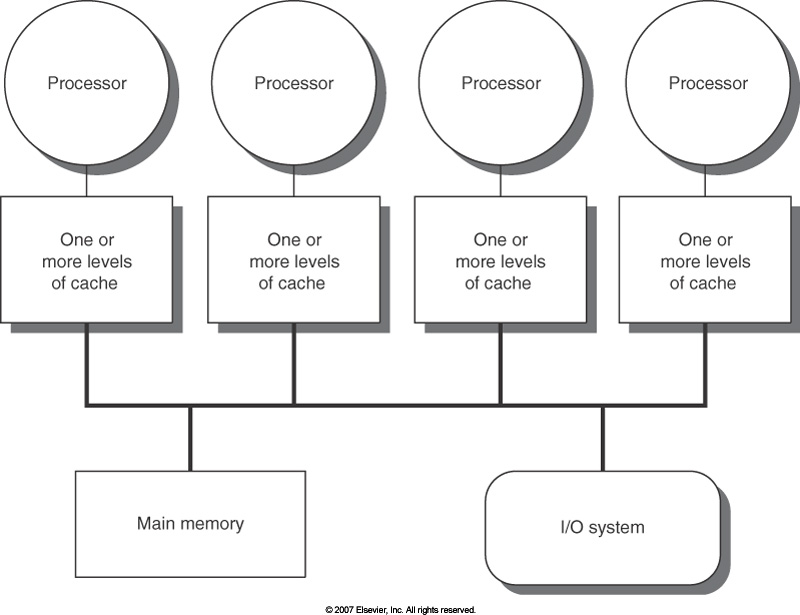
\includegraphics[scale=0.4]{shared_memory.jpg}
\caption{Shared memory Architecture}
\label{Shared memory architecture}
\end{figure}

 All working threads work on the same address space and accessing a memory location previously modified by another processor can be as simple as an access to any other variable. This makes programming in shared memory architectures seem easy, but concurrent access from different processors on the same memory location can lead to unexpected results if not a synchronization scheme is not used. Moreover, shared memory architectures wont typically scale beyond a few thousand nodes, because the bush and memory bandwidth cannot keep up with the increased traffic.

\subsection{Distributed memory}

In distributed memory architectures, every processor has it's own cache and local memory, and it has access only to that memory hierarchy.  All processors are connected on an intercontection network(Ethernet, Mirinet), consist of complex switching topologies. Communication is done using messages from processor to processor and usually being served by memory controller with direct memory access(DMA). Accessing data stored on memory outside the processor, may require several messages to be past between nodes.

%eikona gia distributed

\begin{figure}
 \centering
  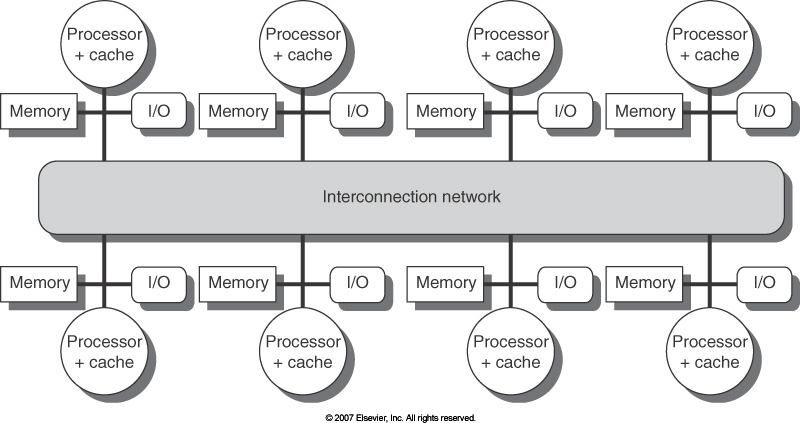
\includegraphics[scale=0.4]{distributed_memory.jpg}
\caption{Distributed memory Architecture}
\label{Distributed memory architecture}
\end{figure}
Programming in a distributed memory environment can be quite challenged, because memory locations needed by a program may not be accessible locally but have to be requested in advance. Efficient parallelization over distributed memory, requires understanding the memory dependencies of the program ability to effectively distribute memory in advance in a way that will minimize communication between distant processes. However, distributed memory can achieve far greater scalability than shared memory, up to thousands of node that can be dynamically inserted and removed from the network.

\subsection{Hybrid Memory}

\begin{figure}
 \centering
  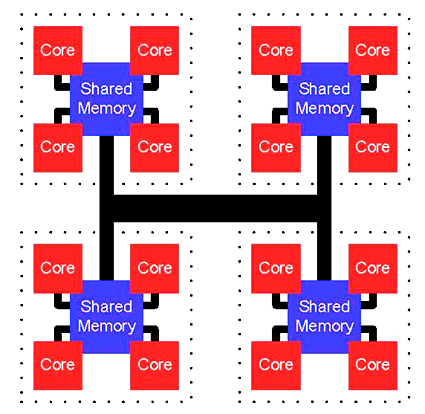
\includegraphics[scale=1.5]{hybrid_memory.jpg}
\caption{Hybrid memory Architecture}
\label{Hybrid memory architecture}
\end{figure}
